Withe the state-space model of the HDT defined, the next step is to design a control strategy that ensures the desired performance. The proposed control strategy is based on a state feedback controller with integral action and resonant states to achieve zero steady-state error for sinusoidal references and disturbances. The block diagram of the proposed control strategy is shown in Fig. \ref{fig:Control_Diagram}.

\begin{equation}
    u_k = -\mathbf{K}_x \mathbf{H}_a
    \begin{bmatrix}
        x_k\\
        m_k
    \end{bmatrix} + \mathbf{K}_{err}e_k - \mathbf{K}_r \rho_k + \mathbf{K}_u m_k
\end{equation}
where $\mathbf{K}_x$ is the state feedback gain matrix, $\mathbf{H}_a$ is the matrix that selects the states without reference, $\mathbf{K}_{err}$ is the error gain matrix, $e_k$ is the error vector, $\mathbf{K}_r$ is the resonant states gain matrix, $\rho_k$ is the resonant states vector, $\mathbf{K}_u$ is the previous control input gain matrix, and $u_{k - 1}$ is the previous control input vector.

\begin{figure}[t!]
    \centering
    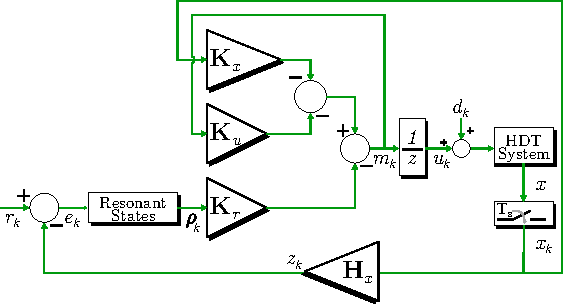
\includegraphics[width=\columnwidth]{Images/Control_Diagram.pdf} 
    \caption{Block diagram of the proposed control strategy for the HDT.}
    \label{fig:Control_Diagram}
\end{figure}

The resonant states are included to ensure zero steady-state error for sinusoidal references and disturbances. The resonant states dynamics are given by:
\begin{equation}
    \dfrac{d\,\rho(t)}{dt} = 
    \underbrace{
    \begin{bmatrix}
        -2\xi\omega & \omega \\
        -\omega & 0
    \end{bmatrix}
    }_{\mathbf{A}_r}
    \rho(t) + 
    \underbrace{
    \begin{bmatrix}
        1\\
        0
    \end{bmatrix}
    }_{\mathbf{B}_r}
    e(t)
\end{equation}
where $\omega$ is the nominal angular frequency, $\xi$ is the damping factor. Each of the references signals has two resonant states associated with it, meaning that for the HDT control, there are eight resonant states in total (4 for the $ev_{cs,\alpha\beta}$ and 4 for the $i_{fp,\alpha\beta}$). This can be expressed as:
\begin{align}
    \dfrac{d\,\rho(t)}{dt} &= \text{blkdiag}(\mathbf{A}_r, \mathbf{A}_r, \mathbf{A}_r, \mathbf{A}_r)\rho(t)\\
    &+ \text{blkdiag}(\mathbf{B}_r, \mathbf{B}_r, \mathbf{B}_r, \mathbf{B}_r)e(t)
\end{align}

These resonant states are then discretized using a ZOH giving the matrices $\mathbf{A}_{rd}$ and $\mathbf{B}_{rd}$. The augmented state-space model of the resonant states can be expressed as:
\begin{align}
    \begin{aligned}
        \begin{bmatrix}
            x_{k + 1}\\
            m_{k + 1}\\
            \rho_{k + 1}
        \end{bmatrix}
        &=
        \begin{bmatrix}
            \mathbf{A}_{d,delay} & \mathbf{0} \\
            \mathbf{B}_{rd}\mathbf{H}_x & \mathbf{A}_{rd}
        \end{bmatrix}
        \begin{bmatrix}
            x_k\\
            m_k\\
            \rho_k
        \end{bmatrix}
        +
        \begin{bmatrix}
            \mathbf{B}_{d,\text{aug}}\\
            \mathbf{0}
        \end{bmatrix}
        \begin{bmatrix}
            u_k\\
            e_k
        \end{bmatrix}
        \\
        y_k &= 
        \begin{bmatrix}
            \mathbf{C} & \mathbf{0}
        \end{bmatrix}
        \begin{bmatrix}
            x_K\\
            m_k\\
            \rho_k
        \end{bmatrix}
    \end{aligned}
\end{align}
where $\mathbf{H}_x$ selects the states from the HDT state vector that are imposed to follow references.

\subsection{Particle Swarm Optimization}

The PSO algorithm is a population-based optimization technique inspired by the social behavior of birds and fish. It consists of a swarm of particles, where each particle represents a potential solution to the optimization problem. The particles move through the search space, updating their positions based on their own experience and the experience of their neighbors. The velocity and position of each particle are updated using the following equations:
\begin{align}
    \begin{aligned}
        v_j(i + 1) &= K_{ap}\left(v_j(i) + c_1 r_1 (pbest_j - x_j(i)) \right.\\
        & \left. + c_2 r_2 (gbest - x_j(i))\right)\\
        x_j(i + 1) &= x_j(i) + v_j(i + 1)
    \end{aligned}
\end{align}
where $v_j(i)$ is the velocity of particle $j$ at iteration $i$, $x_j(i)$ is the position of particle $j$ at iteration $i$, $pbest_j$ is the best position found by particle $j$, $gbest$ is the best position found by the entire swarm, $c_1$ and $c_2$ are cognitive and social acceleration coefficients, $r_1$ and $r_2$ are random numbers uniformly distributed in the range [0, 1], and $K_{ap}$ is the constriction factor given by:
\begin{equation}
    K_{ap} = \dfrac{2}{\left|2 - \phi - \sqrt{\phi^2 - 4\phi}\right|}
\end{equation}
where $\phi = c_1 + c_2 > 4$ is a constant that ensures convergence.

The PSO algorithm iteratively updates the positions and velocities of the particles until a stopping criterion is met, such as a maximum number of iterations or a satisfactory solution. The best position found by the swarm is considered the optimal solution to the optimization problem.